% Options for packages loaded elsewhere
\PassOptionsToPackage{unicode}{hyperref}
\PassOptionsToPackage{hyphens}{url}
%
\documentclass[
  x11names]{article}
\usepackage{amsmath,amssymb}
\usepackage{lmodern}
\usepackage{iftex}
\ifPDFTeX
  \usepackage[T1]{fontenc}
  \usepackage[utf8]{inputenc}
  \usepackage{textcomp} % provide euro and other symbols
\else % if luatex or xetex
  \usepackage{unicode-math}
  \defaultfontfeatures{Scale=MatchLowercase}
  \defaultfontfeatures[\rmfamily]{Ligatures=TeX,Scale=1}
\fi
% Use upquote if available, for straight quotes in verbatim environments
\IfFileExists{upquote.sty}{\usepackage{upquote}}{}
\IfFileExists{microtype.sty}{% use microtype if available
  \usepackage[]{microtype}
  \UseMicrotypeSet[protrusion]{basicmath} % disable protrusion for tt fonts
}{}
\makeatletter
\@ifundefined{KOMAClassName}{% if non-KOMA class
  \IfFileExists{parskip.sty}{%
    \usepackage{parskip}
  }{% else
    \setlength{\parindent}{0pt}
    \setlength{\parskip}{6pt plus 2pt minus 1pt}}
}{% if KOMA class
  \KOMAoptions{parskip=half}}
\makeatother
\usepackage{xcolor}
\usepackage[margin=1in]{geometry}
\usepackage{graphicx}
\makeatletter
\def\maxwidth{\ifdim\Gin@nat@width>\linewidth\linewidth\else\Gin@nat@width\fi}
\def\maxheight{\ifdim\Gin@nat@height>\textheight\textheight\else\Gin@nat@height\fi}
\makeatother
% Scale images if necessary, so that they will not overflow the page
% margins by default, and it is still possible to overwrite the defaults
% using explicit options in \includegraphics[width, height, ...]{}
\setkeys{Gin}{width=\maxwidth,height=\maxheight,keepaspectratio}
% Set default figure placement to htbp
\makeatletter
\def\fps@figure{htbp}
\makeatother
\setlength{\emergencystretch}{3em} % prevent overfull lines
\providecommand{\tightlist}{%
  \setlength{\itemsep}{0pt}\setlength{\parskip}{0pt}}
\setcounter{secnumdepth}{-\maxdimen} % remove section numbering
\usepackage{fontspec} \usepackage{titling} \pretitle{\begin{center} \vspace{-3cm}
\includegraphics[width=\linewidth]{images/Base_info/logo.png}\LARGE\\} \posttitle{\end{center}} \usepackage{float} \usepackage{fancyhdr} \usepackage{ragged2e} \usepackage{caption} \usepackage{colortbl} \captionsetup[figure]{labelformat=empty} \arrayrulecolor{white} \pagestyle{fancy} \fancyhead[L,C]{} \fancypagestyle{plain}{\pagestyle{fancy}} \PassOptionsToPackage{dvipsnames,svgnames*,x11names*}{xcolor} \definecolor{ceil}{rgb}{0.57, 0.63, 0.81} \usepackage[export]{adjustbox} \usepackage{wrapfig} \usepackage{graphicx} \usepackage{caption}
\usepackage{booktabs}
\usepackage{longtable}
\usepackage{array}
\usepackage{multirow}
\usepackage{wrapfig}
\usepackage{float}
\usepackage{colortbl}
\usepackage{pdflscape}
\usepackage{tabu}
\usepackage{threeparttable}
\usepackage{threeparttablex}
\usepackage[normalem]{ulem}
\usepackage{makecell}
\usepackage{xcolor}
\ifLuaTeX
  \usepackage{selnolig}  % disable illegal ligatures
\fi
\IfFileExists{bookmark.sty}{\usepackage{bookmark}}{\usepackage{hyperref}}
\IfFileExists{xurl.sty}{\usepackage{xurl}}{} % add URL line breaks if available
\urlstyle{same} % disable monospaced font for URLs
\hypersetup{
  hidelinks,
  pdfcreator={LaTeX via pandoc}}

\author{}
\date{\vspace{-2.5em}Fecha de creación: 03 April, 2023}

\begin{document}

\setmainfont{Arial}
\setsansfont{Arial}
\setmonofont{Arial}

\newcommand\invisiblesection[1]{%
  \refstepcounter{section}%
  \addcontentsline{toc}{section}{\protect\numberline{\thesection}#1}%
  \sectionmark{#1}}

\fancyhead[R]{\textbf{http://doi.org/10.31687/SaremLR.19.213}}

%
  \refstepcounter{section}%
  \addcontentsline{toc}{section}{\protect\numberline{\thesection}GENERALIDADES}%
  \sectionmark{GENERALIDADES}
\vspace{-0.4cm}


\includegraphics[width=1\linewidth]{images/Base_info/logo}

\vspace{1cm}

\begin{minipage}{0.7\textwidth}
\vspace{0.3cm}
\fontsize{20}{24}\selectfont\textit{Ozotoceros bezoarticus}

\vspace{0.3cm}
\fontsize{30}{36}\selectfont Venado de las pampas
\end{minipage}
\hspace{0.05\textwidth}
\begin{minipage}{0.25\textwidth}

\includegraphics[width=\textwidth]{images/en.png}
\end{minipage}

\normalsize

\begin{figure}[H]

{\centering 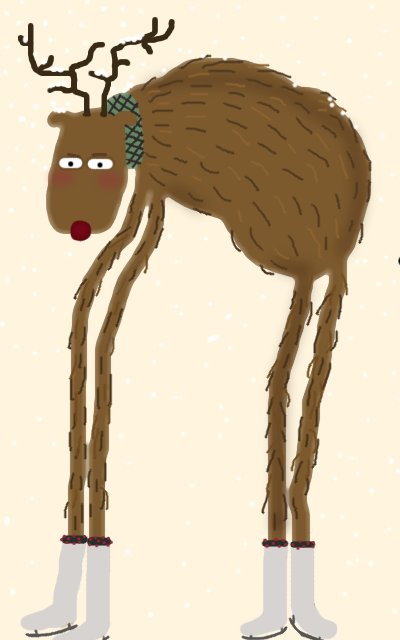
\includegraphics[width=0.35\linewidth]{photos/Blastocerus dichotomus} 

}

\caption{Fotos por Salvador Dali}\label{fig:image}
\end{figure}

\begin{center}\rule{0.5\linewidth}{0.5pt}\end{center}

\justifying

\textbf{Citar como:} Merino, Mariano L.; Cirignoli, Sebastián; Perez
Carusi, Lorena ; Varela, Diego; Kin, Marta Susana; Pautasso, Andres;
Demaría, Manuel; Beade, Mario Santos; Uhart, Marcela. (2019).
\emph{Ozotoceros bezoarticus}. En: SAyDS--SAREM (eds.) Categorización
2019 de los mamíferos de Argentina según su riesgo de extinción. Lista
Roja de los mamíferos de Argentina.
\url{http://doi.org/10.31687/SaremLR.19.213}

\begin{center}\rule{0.5\linewidth}{0.5pt}\end{center}

\newpage

%
  \refstepcounter{section}%
  \addcontentsline{toc}{section}{\protect\numberline{\thesection}ÁREA DE DISTRIBUCIÓN ACTUAL}%
  \sectionmark{ÁREA DE DISTRIBUCIÓN ACTUAL}
\begin{table}[H]
\centering
\begin{tabular}[t]{>{\raggedright\arraybackslash}m{16cm}>{}m{16cm}}
\toprule
\cellcolor{ceil}{\textcolor{white}{\textbf{\rule{0pt}{14pt}ÁREA DE DISTRIBUCIÓN ACTUAL}}}\\
\bottomrule
\end{tabular}
\end{table}

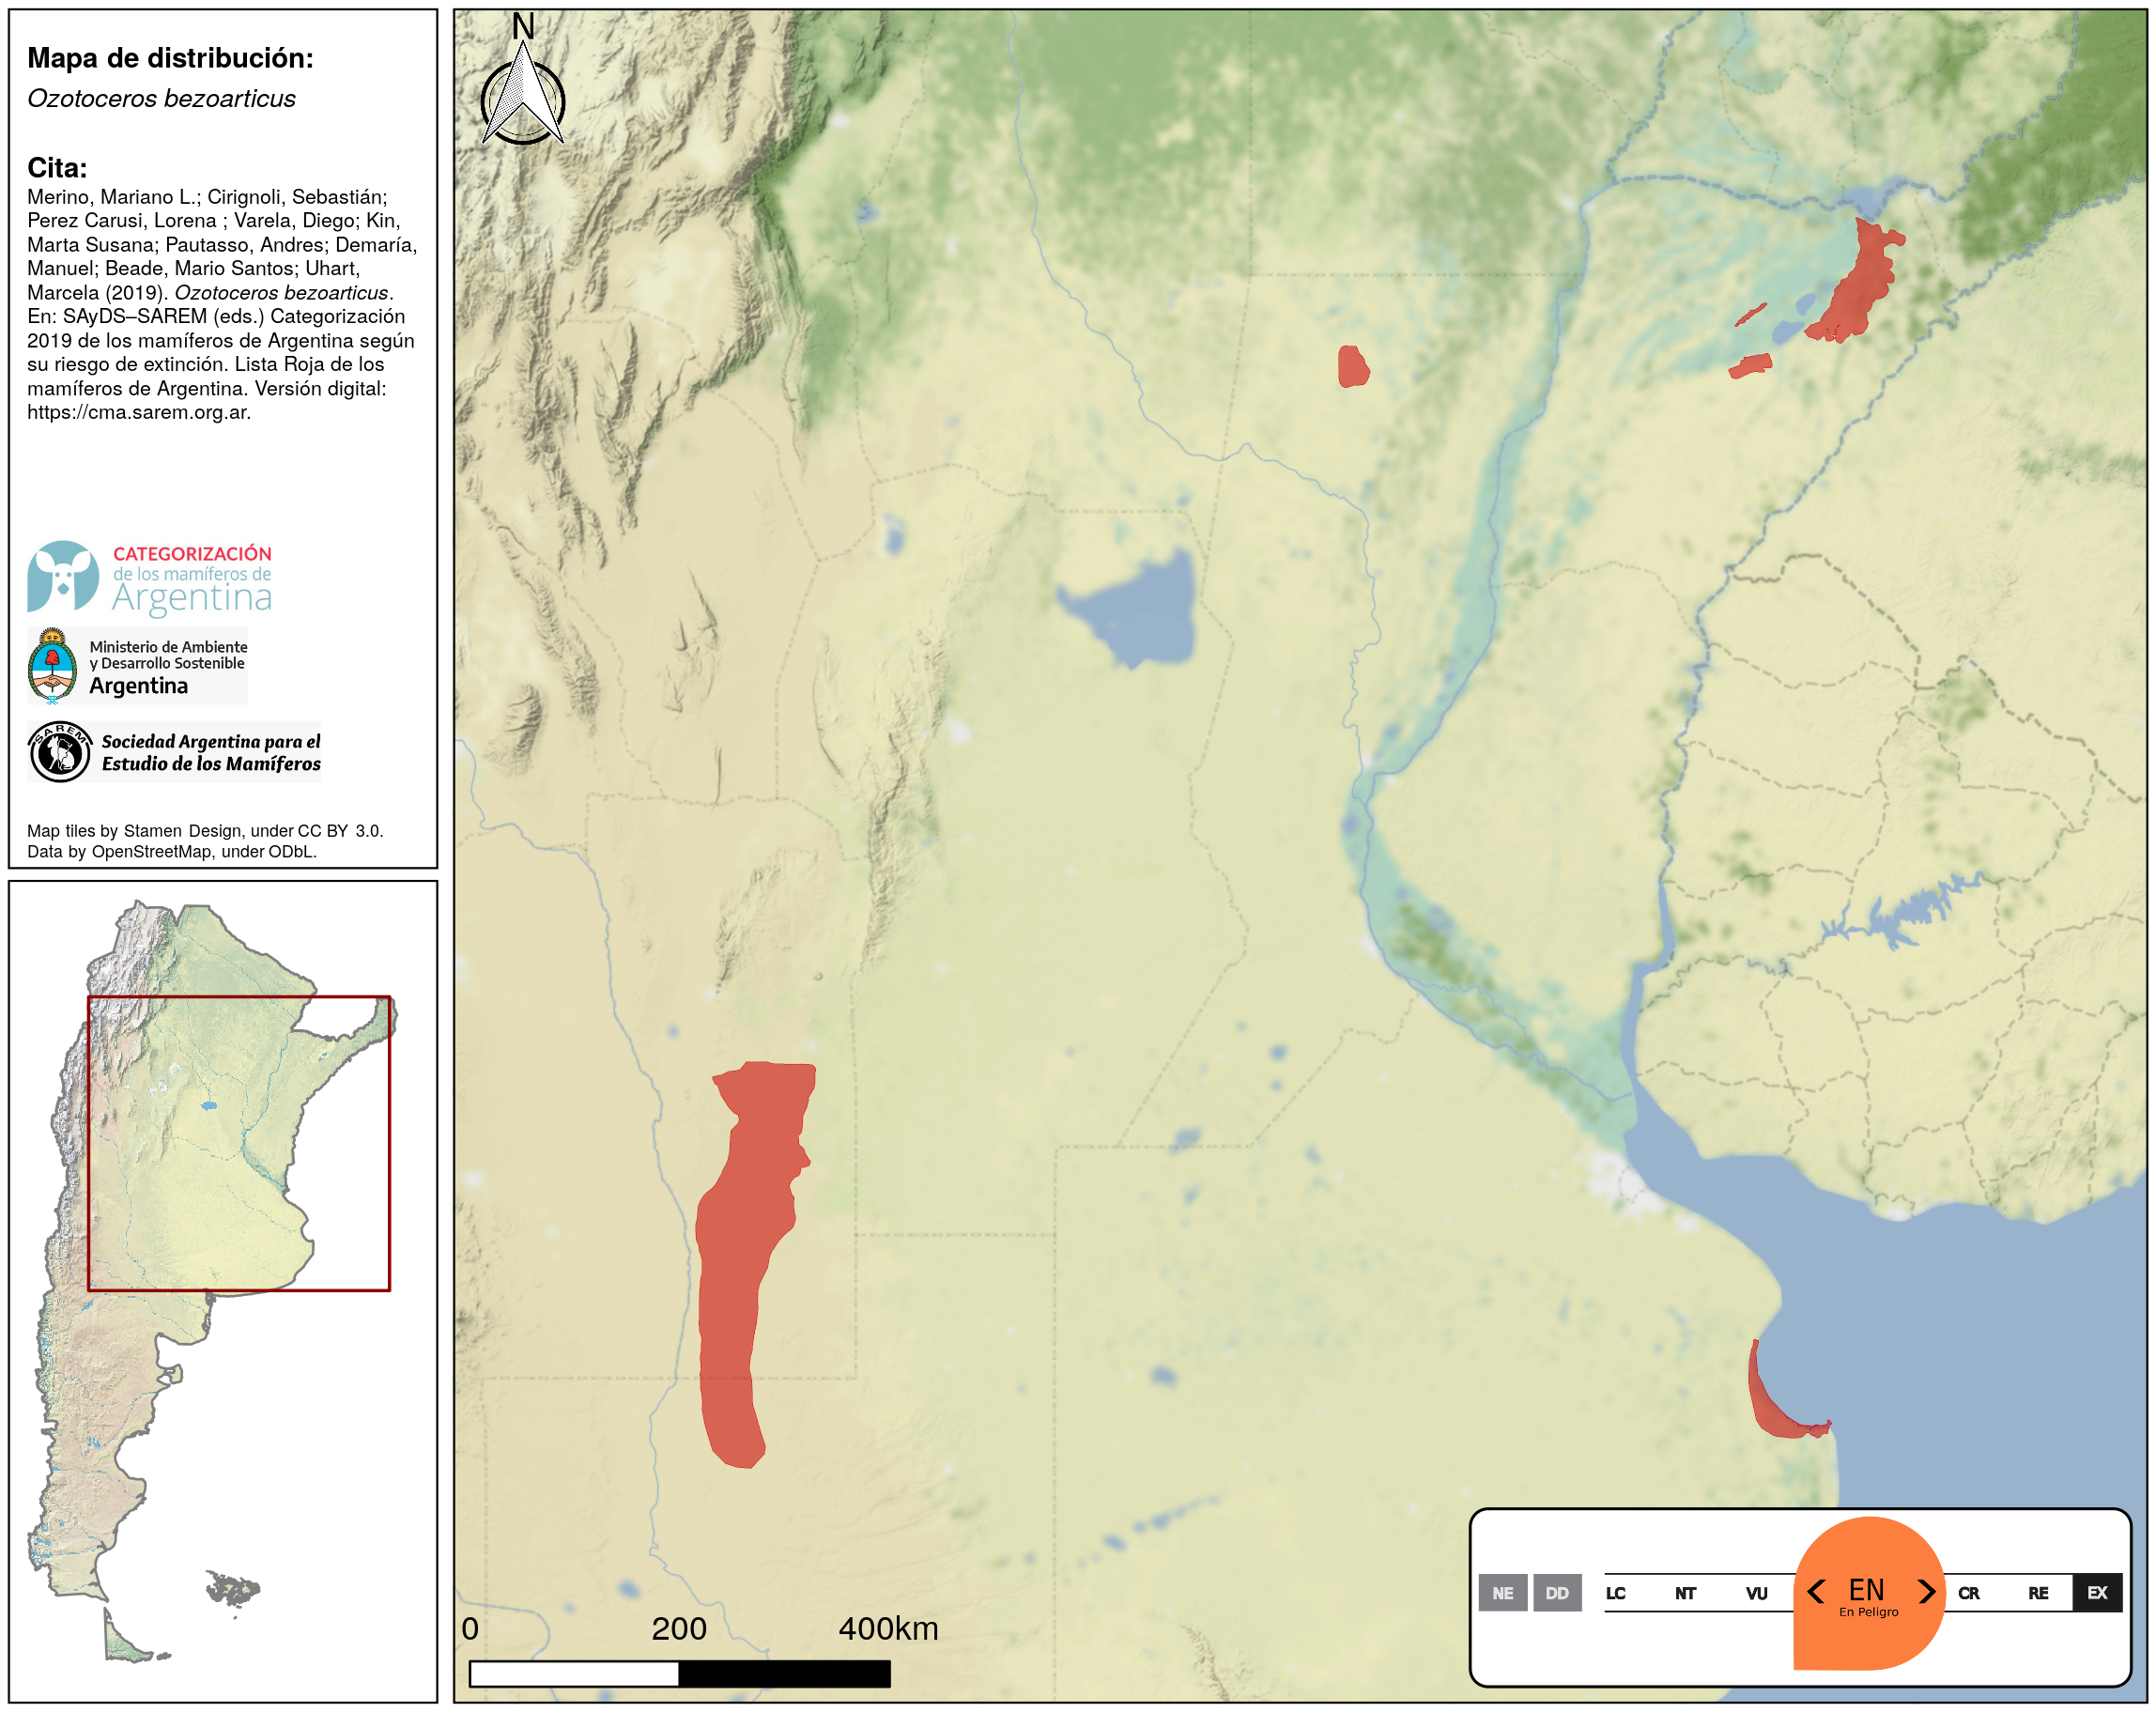
\includegraphics[width=1\linewidth]{maps/Cetartiodactyla/Ozotoceros_bezoarticus}

%
  \refstepcounter{section}%
  \addcontentsline{toc}{section}{\protect\numberline{\thesection}CATEGORÍAS DE CONSERVACIÓN}%
  \sectionmark{CATEGORÍAS DE CONSERVACIÓN}
\begin{table}[H]
\centering
\begin{tabular}[t]{>{\raggedright\arraybackslash}m{16cm}>{}m{16cm}}
\toprule
\cellcolor{ceil}{\textcolor{white}{\textbf{\rule{0pt}{14pt}CATEGORÍAS DE CONSERVACIÓN}}}\\
\bottomrule
\end{tabular}
\end{table}

\vspace{-0.4cm}

\textbf{Categoría Nacional de Conservación 2019}

EN (En Peligro)

\textbf{Criterios y subcriterios}

A3cde

\textbf{Justificación de la categorización}

El venado de las pampas en Argentina, actualmente se encuentra en 4
subpoblaciones aisladas, en Buenos Aires, Corrientes, norte de Santa Fe
y San Luis (incluyendo una pequeña porción de La Pampa). Su población
total se estima en menos de 2.500 individuos maduros, fragmentada en 6
localidades, donde sólo 2 de ellas tienen aproximadamente 1.000
individuos (pastizales de San Luis-La Pampa y cuenca del Aguapey, en
Corrientes). Dos subpoblaciones se consideran En Peligro Crítico (CR),
con menos de 250 individuos adultos (ver evaluación de subpoblaciones
locales). Se proyecta, infiere y sospecha que el tamaño poblacional
puede reducirse más del 50\% en las próximas 3 generaciones
(aproximadamente 20 años, Criterio A3) como consecuencia de la
continuidad e incremento en las amenazas, como la conversión de hábitat
de pastizales en agricultura y plantaciones de pinos (subcriterio c), la
caza furtiva (subcriterio d), la depredación por perros y el impacto de
otras especies exóticas (chancho cimarrón, ciervo axis) (subcriterio e).
Además, mas del 80\% de la población de venados de la Argentina se
encuentra fuera áreas naturales protegidas. Por estos motivos, se
considera que la categoría de conservación a nivel nacional es En
Peligro (EN).

\textbf{Evaluación de subpoblaciones locales}

\begin{tabu} to \linewidth {>{\raggedright}X>{\raggedright}X>{\raggedright}X}
\toprule
\textbf{Subpoblación} & \textbf{Categoría} & \textbf{Criterios y subcriterios}\\
\arrayrulecolor{white}
\midrule
\cellcolor{gray!6}{Buenos Aires} & \cellcolor{gray!6}{CR (En Peligro Crítico)} & \cellcolor{gray!6}{C2a(ii)}\\
\bottomrule
\end{tabu}

\textbf{Justificación}

La población de la provincia de Buenos Aires se encuentra en disminución
desde hace 3 décadas, actualmente se estima que quedan menos de 200
individuos maduros (C2) con una disminución continua, inferida y
proyectada (subcriterio a), como consecuencia de la competencia y/o
depredación por especies de mamíferos exóticos (ciervos Axis, chancho
cimarrón y perros) y por la caza furtiva. A pesar de los esfuerzos de
conservación realizados en las últimas décadas, estas amenazas se hallan
en aumento. El 100\% de la subpoblación de Buenos Aires se encuentra
concentrada en una sola localidad (Bahía Samborombón). La mayor parte de
la población se encuentra fuera del área mejor protegida (PN Campos del
Tuyú).\vspace{0.5cm}

\begin{tabu} to \linewidth {>{\raggedright}X>{\raggedright}X>{\raggedright}X}
\toprule
\textbf{Subpoblación} & \textbf{Categoría} & \textbf{Criterios y subcriterios}\\
\arrayrulecolor{white}
\midrule
\cellcolor{gray!6}{San Luis/La Pampa} & \cellcolor{gray!6}{EN (En Peligro)} & \cellcolor{gray!6}{C2a(ii)}\\
\bottomrule
\end{tabu}

\textbf{Justificación}

Esta población, junto a la de Corrientes, es la más importante del país
en términos poblacionales.~Habita los pastizales pampeanos semi-áridos
de San Luis y La Pampa (donde fue redescubierta recientemente). En el
área con mayor densidad de venados en San Luis, se calculó una población
de más de 700 individuos (Merino et al.~2011, Denápole L., com. pers.) y
se estima que toda la subpoblación está por debajo del umbral de 2.500
individuos maduros (criterio C). Con una disminución continua proyectada
como consecuencia de la pérdida y degradación del hábitat (avance de la
agricultura), caza furtiva, depredación por perros y atropellamientos en
rutas. Se estima que el 95\% de la población se encuentra en solo una
localidad. No se encuentra amparada en áreas naturales
protegidas.\vspace{0.5cm}

\begin{tabu} to \linewidth {>{\raggedright}X>{\raggedright}X>{\raggedright}X}
\toprule
\textbf{Subpoblación} & \textbf{Categoría} & \textbf{Criterios y subcriterios}\\
\arrayrulecolor{white}
\midrule
\cellcolor{gray!6}{Santa Fe} & \cellcolor{gray!6}{CR (En Peligro Crítico)} & \cellcolor{gray!6}{A4bcde+C2a(i,ii)+D}\\
\bottomrule
\end{tabu}

\textbf{Justificación}

Población relictual muy pequeña, con un tamaño sospechado inferior a los
50 individuos maduros y restringidos a una sola localidad (Criterios C2
y D), en la cual se infiere una reducción pasada y proyectada a futuro
mayor al 80\% en el EOO, AOO y en el número de individuos maduros
(Criterio A4). Es la subpoblación menos conocida. Se sospecha que se
encuentra bajo presión de caza furtiva, pérdida de hábitat, depredación
por perros e impacto de eventos extraordinarios de inundaciones. No se
encuentra amparada en áreas naturales protegidas.\vspace{0.5cm}

\begin{tabu} to \linewidth {>{\raggedright}X>{\raggedright}X>{\raggedright}X}
\toprule
\textbf{Subpoblación} & \textbf{Categoría} & \textbf{Criterios y subcriterios}\\
\arrayrulecolor{white}
\midrule
\cellcolor{gray!6}{Corrientes} & \cellcolor{gray!6}{EN (En Peligro)} & \cellcolor{gray!6}{B2ab(ii,iii,v)}\\
\bottomrule
\end{tabu}

\textbf{Justificación}

La subpoblación de Corrientes, en la última década, esta siendo bien
relevada en toda su extensión de presencia (EOO). Se estima que el área
ocupada por la especie es menor a 500 km2 (criterio B2), distribuidos en
tres localidades (subcriterio a). En la localidad principal (Aguapey) se
estimó una población de 1.495 venados (IC 950-2.351) (Zamboni et
al.~2015), pero no se conoce con certeza la tendencia poblacional.~Sin
embargo, se infiere y proyecta una disminución continua (subcriterio b)
como consecuencia del aumento de la conversión de pastizales naturales
en plantaciones forestales de pinos, la degradación de pastizales por
ganadería e invasión de pinos, y por la caza furtiva.~Las otras dos
localidades (San Alonso y Rincón del Socorro) corresponden a núcleos
poblacionales recientemente reintroducidos con poblaciones menores a 150
individuos maduros pero en aumento y se encuentran protegidas dentro del
Parque Nacional Iberá.

\textbf{Categoría Res. SAyDS 1030/04}

EP (En Peligro de Extinción)

\textbf{Categorías nacionales de conservación previas (SAREM)}

\arrayrulecolor{white}

%
  \refstepcounter{section}%
  \addcontentsline{toc}{section}{\protect\numberline{\thesection}TAXONOMÍA Y NOMENCLATURA}%
  \sectionmark{TAXONOMÍA Y NOMENCLATURA}
\begin{table}[H]
\centering
\begin{tabular}[t]{>{\raggedright\arraybackslash}m{16cm}>{}m{16cm}}
\toprule
\cellcolor{ceil}{\textcolor{white}{\textbf{\rule{0pt}{14pt}TAXONOMÍA Y NOMENCLATURA}}}\\
\bottomrule
\end{tabular}
\end{table}

%
  \refstepcounter{section}%
  \addcontentsline{toc}{section}{\protect\numberline{\thesection}INFORMACIÓN RELEVANTE PARA LA EVALUACIÓN}%
  \sectionmark{INFORMACIÓN RELEVANTE PARA LA EVALUACIÓN}
\begin{table}[H]
\centering
\begin{tabular}[t]{>{\raggedright\arraybackslash}m{16cm}>{}m{16cm}}
\toprule
\cellcolor{ceil}{\textcolor{white}{\textbf{\rule{0pt}{14pt}INFORMACIÓN RELEVANTE PARA LA EVALUACIÓN}}}\\
\bottomrule
\end{tabular}
\end{table}

%
  \refstepcounter{section}%
  \addcontentsline{toc}{section}{\protect\numberline{\thesection}RANGO GEOGRÁFICO, OCURRENCIA Y ABUNDANCIA Y NOMENCLATURA}%
  \sectionmark{RANGO GEOGRÁFICO, OCURRENCIA Y ABUNDANCIA Y NOMENCLATURA}
\begin{table}[H]
\centering
\begin{tabular}[t]{>{\raggedright\arraybackslash}m{16cm}>{}m{16cm}}
\toprule
\cellcolor{ceil}{\textcolor{white}{\textbf{\rule{0pt}{14pt}RANGO GEOGRÁFICO, OCURRENCIA Y ABUNDANCIA Y NOMENCLATURA}}}\\
\bottomrule
\end{tabular}
\end{table}

%
  \refstepcounter{section}%
  \addcontentsline{toc}{section}{\protect\numberline{\thesection}DATOS MORFOMÉTRICOS}%
  \sectionmark{DATOS MORFOMÉTRICOS}
\begin{table}[H]
\centering
\begin{tabular}[t]{>{\raggedright\arraybackslash}m{16cm}>{}m{16cm}}
\toprule
\cellcolor{ceil}{\textcolor{white}{\textbf{\rule{0pt}{14pt}DATOS MORFOMÉTRICOS}}}\\
\bottomrule
\end{tabular}
\end{table}

%
  \refstepcounter{section}%
  \addcontentsline{toc}{section}{\protect\numberline{\thesection}RASGOS ETO-ECOLÓGICOS}%
  \sectionmark{RASGOS ETO-ECOLÓGICOS}
\begin{table}[H]
\centering
\begin{tabular}[t]{>{\raggedright\arraybackslash}m{16cm}>{}m{16cm}}
\toprule
\cellcolor{ceil}{\textcolor{white}{\textbf{\rule{0pt}{14pt}RASGOS ETO-ECOLÓGICOS}}}\\
\bottomrule
\end{tabular}
\end{table}

%
  \refstepcounter{section}%
  \addcontentsline{toc}{section}{\protect\numberline{\thesection}CONSERVACIÓN E INVESTIGACIÓN}%
  \sectionmark{CONSERVACIÓN E INVESTIGACIÓN}
\begin{table}[H]
\centering
\begin{tabular}[t]{>{\raggedright\arraybackslash}m{16cm}>{}m{16cm}}
\toprule
\cellcolor{ceil}{\textcolor{white}{\textbf{\rule{0pt}{14pt}CONSERVACIÓN E INVESTIGACIÓN}}}\\
\bottomrule
\end{tabular}
\end{table}

%
  \refstepcounter{section}%
  \addcontentsline{toc}{section}{\protect\numberline{\thesection}BIBLIOGRAFÍA}%
  \sectionmark{BIBLIOGRAFÍA}
\begin{table}[H]
\centering
\begin{tabular}[t]{>{\raggedright\arraybackslash}m{16cm}>{}m{16cm}}
\toprule
\cellcolor{ceil}{\textcolor{white}{\textbf{\rule{0pt}{14pt}BIBLIOGRAFÍA}}}\\
\bottomrule
\end{tabular}
\end{table}

\newpage

%
  \refstepcounter{section}%
  \addcontentsline{toc}{section}{\protect\numberline{\thesection}AUTORES}%
  \sectionmark{AUTORES}
\begin{table}[H]
\centering
\begin{tabular}[t]{>{\raggedright\arraybackslash}m{16cm}>{}m{16cm}}
\toprule
\cellcolor{ceil}{\textcolor{white}{\textbf{\rule{0pt}{14pt}AUTORES}}}\\
\bottomrule
\end{tabular}
\end{table}

\textbf{AUTORES}

\begin{tabu} to \linewidth {>{}l>{\raggedright\arraybackslash}p{2cm}>{\raggedright}X}
\toprule
\textbf{\cellcolor{gray!6}{Beade, Mario Santos}} & \cellcolor{gray!6}{} & \cellcolor{gray!6}{Parque Nacional Campos del Tuyú, Administración de Parques Nacionales, General Lavalle, Buenos Aires, Argentina}\\
\textbf{Cirignoli, Sebastián} &  & Centro de Investigaciones del Bosque Atlántico (CeIBA), Puerto Iguazú, Misiones, Argentina\\
\textbf{\cellcolor{gray!6}{Demaría, Manuel}} & \cellcolor{gray!6}{} & \cellcolor{gray!6}{Estación Experimental Agropecuaria San Luis, INTA, Villa Mercedes, San Luis, Argentina}\\
\textbf{Kin, Marta Susana} &  & Facultad de Ciencias Exactas y Naturales, Universidad Nacional de La Pampa, Santa Rosa, La Pampa, Argentina\\
\textbf{\cellcolor{gray!6}{Merino, Mariano L.}} & \cellcolor{gray!6}{} & \cellcolor{gray!6}{Centro de Bioinvestigaciones, Centro de Investigaciones y Transferencia del Noroeste de la Provincia de Buenos Aires (CIT-NOBA), UNNOBA-CONICET, Pergamino, Buenos Aires, Argentina}\\
\addlinespace
\textbf{Pautasso, Andres} &  & Museo Provincial de Ciencias Naturales Florentino Ameghino, Santa Fe, Santa Fe, Argentina\\
\textbf{\cellcolor{gray!6}{Perez Carusi, Lorena}} & \cellcolor{gray!6}{} & \cellcolor{gray!6}{Coordinación Regional Centro Este, Administración de Parques Nacionales, Buenos Aires, Argentina}\\
\textbf{Uhart, Marcela} &  & Karen C. Drayer Wildlife Health Center’s Latin America Program, Universidad de California, Davis, , Estados Unidos\\
\textbf{\cellcolor{gray!6}{Varela, Diego}} & \cellcolor{gray!6}{} & \cellcolor{gray!6}{Instituto de Biología Subtropical (IBS), CONICET-Universidad Nacional de Misiones y Centro de Investigaciones del Bosque Atlántico (CeIBA), Puerto Iguazú, Misiones, Argentina}\\
\bottomrule
\end{tabu}

\textbf{COLABORADORES}

\begin{tabu} to \linewidth {>{}l>{\raggedright\arraybackslash}p{2cm}>{\raggedright}X}
\toprule
\textbf{\cellcolor{gray!6}{Denápole, Lara}} & \cellcolor{gray!6}{} & \cellcolor{gray!6}{Área Flora y Fauna, Ministerio de Medio Ambiente, Campo y Producción de la Provincia de San Luis, San Luis, Argentina}\\
\textbf{Iezzi, María Eugenia} &  & Instituto de Biología Subtropical (IBS), CONICET-Universidad Nacional de Misiones y Centro de Investigaciones del Bosque Atlántico (CeIBA), Puerto Iguazú, Misiones, Argentina\\
\bottomrule
\end{tabu}

\end{document}
